% !TEX root = SegwayDoku.tex
\renewcommand{\autoren}{Timo Veit, Aleksandar Stoiljkovic}
\newpage
\section{Dynamik des Roboters}
\subsection{Aufstellen der Differentialgleichungen nach Lagrange}
Durch den Lagrange-Formalismus lassen sich die Bewegungsdifferentialgleichungen des Systems beschreiben. Diese findet hier im Vergleich zur „Newton‘schen Formulierung der Bewegungsgesetze“ bessere Anwendung.

Bevor wir das System mit dem Lagrange-Formalismus gelöst haben, versuchten wir es mit der D'Alembert-Methode. Dieses Vorgehen war uns aus der Technischen Dynamik Vorlesung bekannt. Jedoch bereitete uns diese Vorgehensweise große Probleme und zahlreiche Unbekannte Kräfte, welche wir nicht eliminieren konnten. Das ganze System wurde sehr unübersichtlich und komplex. Aus diesem Grund entschieden wir uns dann für den Lagrange-Formalismus, da äußere Zwangskräfte leichter dargelegt werden können und somit physikalische Probleme vereinfacht werden.
\begin{flalign}
L & = T - V
\end{flalign}
T: gesamte kinetische Energie\newline
V: gesamte potentielle Energie\newline


Die kinetische Energie des Systems setzt sich aus der translatorischen Energie der beiden Räder zuzüglich der roatatorischen Energie der beiden Räder zusammen.
Hinzu kommt die translatorische Energie des Gehäuses(Schwerpunkt) sowie die rotatorische Energie des Gehäuses, welche durch das Kippen entsteht.
Die gesamte kinetische Energie ist somit die Summe aus den einzelnen kinetischen Energien.

Das Nullniveau wurde auf die Radmittelachse gesetzt. Daraus folgt, dass sich die potentielle Energie allein durch die Höhe des Gehäuseschwerpunktes bestimmt.\newline
Für die Berechnungen wurde $\beta$ linearisiert.\newline
Somit gilt im Folgendem: sin($\beta$) = $\beta$ und cos($\beta$) =1 \newline

Desweiteren gilt: ${\beta}^2$ ist nicht linearisierbar. Jedoch ist der Wert sehr klein und kann somit als 0 angenommen werden und wird somit im weiteren Verlauf der Berechnungen nicht berücksichtigt.

\begin{flalign}
L & = T_{Rad1} + T_{Rad2} - V_{Gehaeuse}
\end{flalign}

Hinweis: Sämtliche Formeln für die Auslegung der Dynamik befinden sich in der beigelegten Matlab-Datei.\newline
Name der Dateien: DynamicsLagrange und Dynamikmodell

\newpage
\subsection{Reglerauslegung}
Folgende Regler werden für ein kontrolliertes System benötigt:
\begin{itemize}
	\item Kippregler
	\item Rotationsgeschwindigkeitsregler
	\item Geschwindigkeitsregler
	\item Positionsregler
\end{itemize}
Zunächst muss die Gesamtübertragungsfunktion der einzelnen Reglers aufgestellt werden:
\begin{flalign}
\frac{Vorwaerts}{1-Gesamt}
\end{flalign}

\begin{figure}[!h]  % [h] bedeutet, dass das Bild genau an dieser Stelle im Text erscheint
	% mit width=... wird die Größe des Bildes in Prozent der Seitenbreite eingestellt
	\centering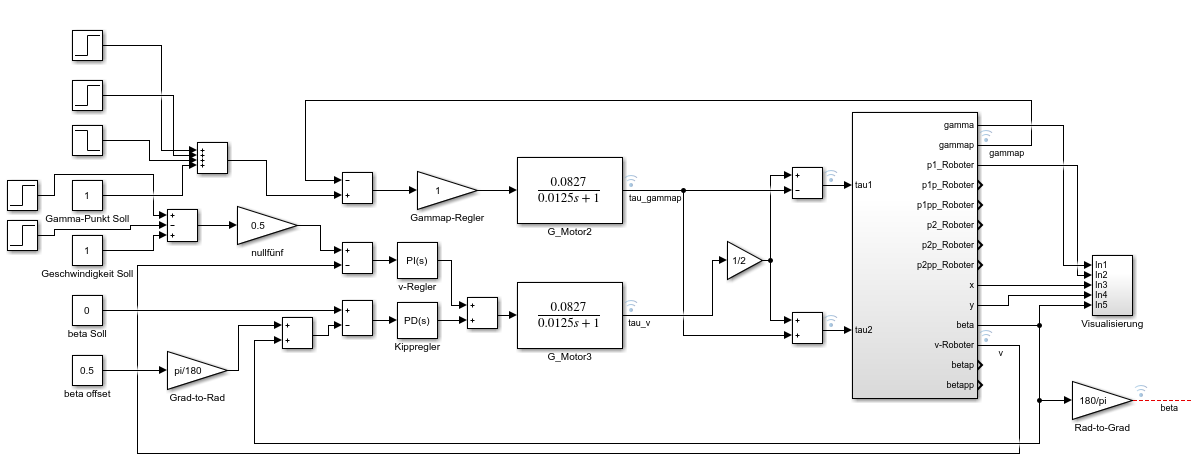
\includegraphics[width=1.0\textwidth]{images/SimulinkReglerstruktur.png}
	% caption ist die Bildunterschrift, taucht auch im Abbildungsverzeichnis auf
	\caption{Simulinkmodell \newline(Quelle: Eigenes Modell)}
	\label{bild_1.1} % über das label kann man aus dem Text auf das Bild verweisen
\end{figure}

Das Wurzelortskurvenverfahren zum Entwerfen der Regler bietet sich an, da das gegebene System an das Zeitverhalten des geschlossenen Kreises sowie der Lage des dominierenden Polpaares gebunden ist.  Dabei wird die Übertragungsfunktion des offenen Kreises $G_{Strecke}(s)\cdot G_{Regler}(s)$ gebildet und die entsprechende Wurzelortskurve betrachtet. Aus dem qualitativen Verlauf der Wurzelortskurve ist bekannt, wie sich die Pole, in Abhängigkeit der Reglerverstärkung k, verändern. Sie liegen für k=0 im Ursprung ihres Astes und bewegen sich für steigende Verstärkungen an ihm entlang, bis sich der Pol für k→ ∞ im Unendlichen befindet oder durch eine in der Nähe befindliche Nullstelle kompensiert wird. Letztendlich müssen dem Regler eine oder mehrere Nullstellen gegeben werden, welche die Äste der Wurzelortskurven des offenen Kreises verändern. Dadurch soll das dominierende Polpaar durch eine bewusste Wahl der Reglerverstärkung k in den gewünschten Bereich der komplexen Ebene gelangen und damit das System stabilisieren. Im Optimalfall werden dadurch die restlichen Polstellen so weit nach links verschoben, dass sie einen möglichst geringen Einfluss auf das System haben und das dominierende Polpaar alleine das Verhalten bestimmt.

\subsubsection{Kippregler}
Der Kippregler sorgt dafür, dass der Roboter sowohl während der Fahrt, als auch im Stand in einer stabilen Lage bleibt und nicht umkippt.
Verwendet wurde hierfür ein PD - Regler.

Die Koeffizienten lauten:
P = -18,88
D = -1,33
\subsubsection{Rotationsgeschwindigkeitsregler}
Für den Rotationsgeschwindigkeitsregler wurde ein einfacher P-Regler verwendet. Die Verstärkung muss in einem Experiment getestet werden.
\subsubsection{Geschwindigkeitsregler}
Der Geschwindigkeitsregler wird benötigt, um den Sollwert der Geschwindigkeit schnell und möglichst genau zu erreichen und späteren Verlauf zu halten.
Verwendet wurde ein PI - Regler.
P = -6,05
I = -6,05
\subsubsection{Positionsregler}
Nachdem der Roboter seine vorgegeben Koordinaten erreicht hat, soll er diese auch halten und dafür sorgt der Positionsregler.
Verwendet wurde ein 

